\section{Installation}
\label{installation}

Start off by downloading \bms~for your operating system. 
You can find the latest version of the tool at \url{http://www.stups.hhu.de/ProB/index.php5/BMotion_Studio}.
Decompress the archive and expand the directory if necessary. 

%\warning{Do not change the location and structure of the files and directories within the folder!}

Navigate to the \texttt{bin} folder and start the tool by entering the bash command:

\begin{lstlisting}[language=bash]
.\bmotion-prob
\end{lstlisting}

\info{Windows users should execute the \texttt{bmotion-prob.bat} file.}

That's all! 
Your default browser should open and show the default workspace.
The workspace contains the following predefined folders:

\begin{itemize}
\item \texttt{libs}: This folder contains JavaScript libraries that are needed for BMotion Studio.
\item \texttt{b\_template}: A visualisation template for creating visualisations for Classical-B and Event-B models.
\item \texttt{csp\_template}: A visualisation template for creating visualisations for CSP models.
\end{itemize}

\section{Creating a new Visualisation Template}
\label{vis_template}

%Let's start by creating a new visualisation template.
The easiest way to create a new visualisation template is to duplicate one of the default templates  \texttt{b\_template} (for Event-B or Classical-B visualisations) or \texttt{csp\_template} (for CSP-M visualisations) that are included in the \texttt{workspace} folder of your \bms~installation.
Just duplicate the folder.
After refreshing your browser, the newly created folder should appear in your workspace.
Navigate to the folder. 
The folder contains three files.

\paragraph{\texttt{template.groovy:}}
The Groovy script file is the place where the user can communicate with the formal model by means of the ProB Java API\footnote{\url{http://www.stups.hhu.de/ProB/index.php5/ProB_Java_API}}.
For instance, the user may register methods that can be called in the JavaScript file.
%The Groovy script file is the place where you can setup the communication between your visualisation and the ProB animator.
%In particular, the Groovy script file is the link between the formal model and the visualisation.
%It allows you to programmatically control the ProB animator and to access the actual formal model being visualised.

\paragraph{\texttt{template.js:}}
In the JavaScript file you can setup observers and actions.
Moreover, the user can take advantage of the entire JavaScript language.
There exist are a lot of libraries for JavaScript that you can apply to create custom visualisations.
For instance, it exists libraries for manipulating the DOM of an HTML document, or for generating chart and plot diagrams.
%In addition, you can call functions that are registered in the Groovy script file.
%This enables you to add some interactivity to your visualisation.
%For instance, pressing a button in your visualisation could cause the execution of an Event-B event.
Here is an example JavaScript file:

\begin{lstlisting}[language=JavaScript]
require(['prob'], function (prob) {
  // Put your code here
});
\end{lstlisting}

The \textit{prob} parameter is the access point to the BMotion Studio for ProB API.

\paragraph{\texttt{template.html:}}
The HTML file is the root file of your visualisation. It contains the actual visualisation and it's configuration.
Here is an example HTML file:

\begin{lstlisting}[language=html]
<html bms-app>
  <head>
      <title>BMotion Studio for ProB</title>
      <meta name="bms.tool" content="BAnimation" />
      <meta name="bms.script" content="template.groovy" />
      <script src="/bms/libs/requirejs/require.js"></script>
      <script>
        require(['/bms/libs/prob/config.js'], function () {
          require(['template']);
        });
      </script>
  </head>
  <body>
  </body>
</html>
\end{lstlisting}

The meta tag \textit{bms.tool} (line 4) defines the formalism or the simulator respectively that should be used. 
Two values are allowed: ``BAnimation'' for creating visualisations of Event-B or Classical-B models and ``CSPAnimation'' for creating visualisations of CSP-M models.
The meta tag \textit{bms.script} (line 5) contains the link to the Groovy script file.
Finally, in line 9 we define the path to the JavaScript file.

The user is not restricted to an editor in order to create a visualisation.
The user can make use of any tool that support the creation of SVG graphics or HTML documents.
For the tutorials (Section~\ref{tutorial_b} and~\ref{tutorial_csp}) we are going to use the Inkspace\footnote{\url{https://inkscape.org}} editor. Inkscape is an editor for creating vector graphics that is available for Windows, Mac OS X and Linux.
It's free and open source.
With Inkscape the user can export the vector graphic into the SVG format.

\begin{figure}[!ht]
\begin{center}
	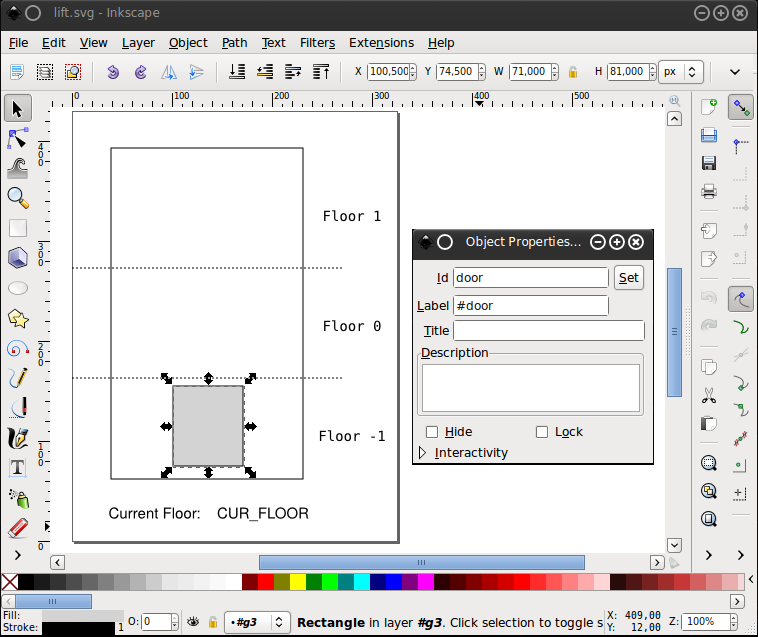
\includegraphics[width=12cm]{img/tutorial/tut_02.png}
	\caption{Creating an SVG graphic with Inkscape}
	\label{fig_tut_02_inkscape}
\end{center}
\end{figure} 


\section{Linking a Model with the Visualisation}

In order to link a model with a visualisation, open the HTML file with an HTML/text editor of your choice and add the following line within the head tag, where XXX is the relative path to your model file (e.g. ``model/my-model.mch''):

\begin{lstlisting}[language=html]
<meta name="bms.model" content="XXX" />
\end{lstlisting}

Linking a model within the html file automatically loads the model, when starting the visualisation.

To create a link between visual elements and the model, please checkout the Section about observers (\ref{tutorial_b} for Event-B and Classical-B or \ref{tutorial_csp} for CSP).
